\documentclass{article}
\usepackage{graphicx} % Required for inserting images
\usepackage{float}
\usepackage{amsmath}

\title{ECE148: Signal Processing Applications \\ \large
        Assignment 7: Range and Bearing-Angle Estimation}
\author{Andy Chen}
\date{May 2026}

\begin{document}

\maketitle

\section*{Part A: Bearing-Angle Estimation}
A passive detector consists of two acoustic receivers. The separation between the receivers is \textit{2.0 meters}. The acoustic propagation speed in air is \textit{343.6 m/s}. The sampling rate of the A/D conversion is \textit{48 kHz}.

\subsection*{Cross-Correlation and Time-Delay Estimation}
We perform cross-correlation of the two data tracks. Cross-correlation measures the similarity between the two signals as one signal is shifted relative to the other. The discrete cross-correlation is defined as:
\[
R_{xy}[k] = \sum_n=x[n] \ y[n-k]
\]
where \(x[n]\) and \(y[n]\) are sampled acoustic signals, and \(k\) is the lag variable in samples. The peak of the cross-correlation function corresponds to the lag value that produces the greatest similarity between the two signals. Because the lag is measured in samples, it must be converted into a physical time delay using the sampling frequency \(f_s=48\) kHz:
\[
\tau=\frac{k}{f_s}
\]
\begin{figure}[H]
    \centering
    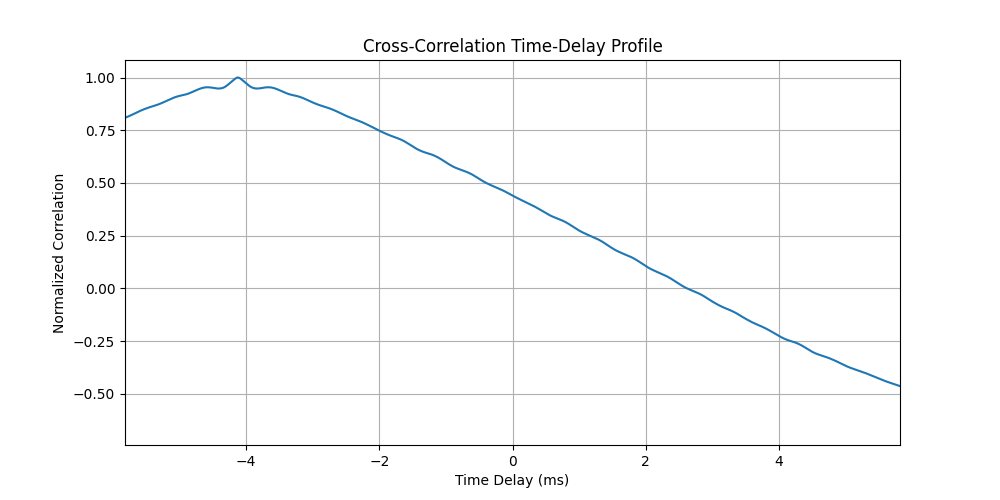
\includegraphics[width=1\linewidth]{crosscorrelation_timedelay.png}
    \caption{Plot of the resultant correlation function as the time-delay profile (estimate of the time-delay).}
\end{figure}

\subsection*{Bearing Angle Estimation}
We convert the time delay estimation into a bearing angle using the geometry of the receiver arrangement. For a receiver spacing \(d\) and sound propagation speed \(c\), the relationship between the time delay \(\tau\) and bearing angle \(\theta\) is:
\[
\tau=\frac{d\sin(\theta)}{c}
\]
Solving for the bearing angle provides:
\[
\theta=\sin^{-1}\bigg(\frac{c\tau}{d}\bigg)
\]
Only delays satisfying \(|\frac{c\tau}{d}|=1\) are physically valid, since the argument of inverse sine must remain within the interval \([-1,1]\).

\begin{figure}[H]
    \centering
    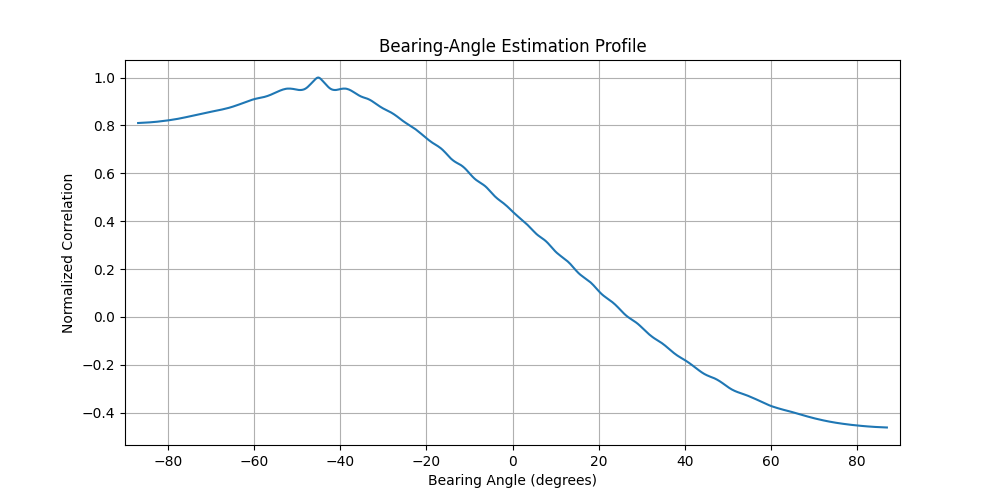
\includegraphics[width=1\linewidth]{bearing_angle_estimation.png}
    \caption{Plot of the bearing-angle estimation profile of the acoustic source as a function of the angle.}
\end{figure}

\section*{Part B: 5-Gun Salute}
Given a single-channel (mono) soundtrack, we produce a stereo soundtrack such that, with headphones, the sound source moves from \(-60^{\circ}\) to \(+60^{\circ}\) in 5 steps, at \(-60^{\circ},-30^{\circ},0^{\circ},+30^{\circ}\), and \(+60^{\circ}\) sequentially.

\subsection*{Approach and Implementation}
The implementation uses interaural time difference (ITD) to simulate binaural localization cues. Essentially, human listeners localize sound partly by detecting small differences in arrival time between the two ears. If a source is located on the left side, the sound reaches the left ear slightly earlier, and reaches the right ear slightly later. Similarly, right-side sources arrive earlier at the right ear.
\\
\\
For a source located at angle \(\theta\), the interaural delay is approximately:
\[
\tau=\frac{d\sin(\theta)}{c}
\]
where \(d\) is the ear spacing, \(c\) is the speed of sound, and \(\theta\) is the source angle. We implement this delay digitally by delaying one stereo channel relative to the other.

\subsection*{Implementation and Results}
Assuming an ear spacing of \(d=0.20\) m, we compute the interaural delay \(\tau\) for each angle \(\theta\). The delay was then converted into samples \(N=\tau f_s\) where \(f_s\) is the sampling frequency. For negative angles, the right channel was delayed. For positive angles, the left channel was delayed. At zero degrees, no delay was applied. The stereo version of the entire audio sample was generated independently for each angle. The five processed stereo signals were then concatenated sequentially to form the final stereo output.
\\
\\
The generated soundtrack successfully created the perception of a moving sound source when played through headphones. Each repetition of the audio sample was played at the distinct locations \(\theta\in[-60^{\circ},-30^{\circ},0,+30^{\circ},+60^{\circ}]\). The localization effect was produced entirely through interaural time difference cues. The delayed arrival at one ear caused the listener's auditory system to interpret the sound as originating from the corresponding direction.

\section*{Part C: Range Estimation}
We perform step-frequency FMCW radar imaging using FFT for range estimation. The given dataset was taken over a section of the walkway pavement in front of Broida Hall. The ground-penetrating radar imaging unit scanned along a linear path and took data at 200 spatial positions. The spatial spacing between the data-collection points was 0.0213 m. At each data-collection position, the system illuminated the subsurface region of the walkway area with microwaves in the step-frequency (FMCW) mode, stepping through 128 frequencies with a constant increment, from 0.976 GHz to 2.00 GHz. The relative permittivity \(\epsilon_r\) is approximately 6.0. The dataset is in the form of a \(200\times128\) array, corresponding to 128 complex-amplitude values (for the 128 frequencies) at 200 data-acquisition points.

\subsection*{GPR Imaging Implementation}
We load the data and extract the following variables:
\begin{itemize}
    \item \textbf{F}: complex FMCW frequency-domain data array.
    \item \textbf{f}: transmit frequency vector.
    \item \textbf{da}: antenna position vector.
\end{itemize}
Since the radar wave propagates through pavement rather than free space, the propagation velocity was adjusted using the relative permittivity:
\[
v=\frac{c}{\sqrt{\epsilon_r}}\approx1.225\times10^8
\]
The measured data was sampled in the frequency domain. To obtain depth information, we perform an IFFT along the frequency dimension \(f\). Zero-padding was applied before the IFFT to improve interpolation and visualization smoothness, in this case \(N_{FFT}=2048\). The magnitude of the IFFT result was then computed to form the radar intensity image.
\\
\\
The FMCW radar frequency spacing determines the delay resolution:
\[
dt = \frac{1}{\Delta f \cdot N_{FFT}}
\]
The corresponding depth axis was computed using:
\[
d=\frac{vt}{2}
\]
where the factor of 2 accounts for the round-trip propagation path between the antenna and the subsurface reflector.
\\
\\
Because radar reflections span a large dynamic range, we applied logarithmic compression to the image. This improved the visibility of weaker reflections, such as the rebars. The display range was clipped from \(-40\) to 0 dB to improve image contrast.

\subsection*{Resolution Limit and Maximum Detectable Depth}
The depth resolution of the FMCW radar system is determined by the total bandwidth:
\[
\Delta d = \frac{v}{2B}
\]
Because the bandwidth was between 2.00 GHz and 0.976 GHz, we have \(B=1.024\) GHz. Substituting the propagation delay and bandwidth, we have:
\[
\Delta d\approx0.0598 \text{ m}
\]
Thus, the depth resolution limit is approximately 6.0 cm.
\\
\\
The maximum detectable depth is determined by the frequency spacing:
\[
\Delta f=\frac{B}{128} = 8.0 \text{ MHz}
\]
The maximum measureable delay is:
\[
t_{max} = \frac{1}{\Delta f} = 1.25\times10^{-7} \text{ s}
\]
Converting to depth, we have:
\[
d_{max} = \frac{vt_{max}}{2} \approx 7.66 \text{ m}
\]
Thus, the maximum depth is approximately 7.7 m.

\subsection*{Physical Pixel Size}
Using the antenna spacing, we have that the horizontal pixel size is 0.0213 m/pixel or 2.13 cm/pixel. The vertical pixel spacing after zero padding can be determined from the depth axis:
\[
dz =depth[1] - depth[0]
\]
Using the reconstruction parameters, we find that the vertical pixel size is approximately 0.37 cm/pixel.

\begin{figure}[H]
    \centering
    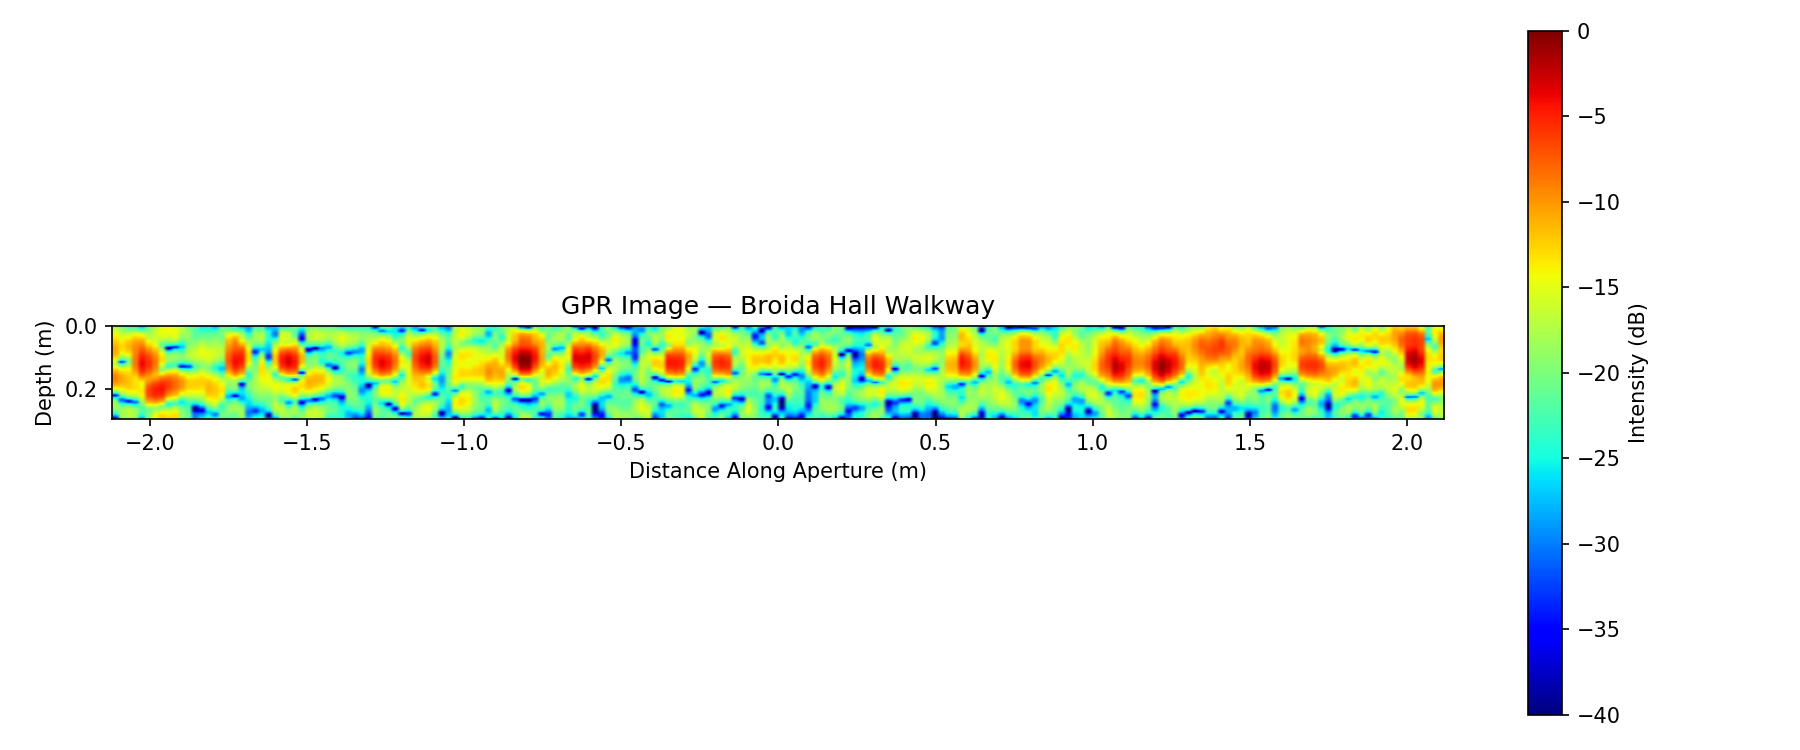
\includegraphics[width=1\linewidth]{gpr_image.png}
    \caption{Image reconstruction of the subsurface profile.}
\end{figure}

\subsection*{Summary}
We processed step-frequency FMCW radar data to reconstruct a subsurface image of the pavement in front of Broida Hall. An inverse FFT was applied along the frequency dimension to generate depth profiles corresponding to each antenna position. The radar propagation velocity was adjusted using the relative permittivity of the pavement material, and the resulting delay profiles were converted into physical depth using the round-trip propagation relationship. The final reconstructed image successfully revealed subsurface reflections corresponding to rebars and other shallow features beneath the pavement.

\end{document}
